\documentclass[UTF8]{ctexart}
\usepackage[paper=a4paper,dvips,top=2.5cm,left=2.8cm,right=2.8cm,foot=1cm,bottom=3.2cm]{geometry}
\usepackage{fancyhdr}
\usepackage{indentfirst}
\usepackage{enumerate}
\usepackage{clrscode}
\usepackage{listings}
\lstset{language=Matlab}%代码语言使用的是matlab
\lstset{breaklines}%自动将长的代码行换行排版
\lstset{extendedchars=false}%解决代码跨页时,章节标题,页眉等汉字不显示的问题
\usepackage{graphicx}
\DeclareGraphicsExtensions{.eps,.ps,.jpg,.bmp}
\pagestyle{plain}
\author{王超民$\;\;$1502120796}
\title{统计学习作业}
\begin{document}
\maketitle
\section*{利用SVM做人脸识别}
\subsection*{实验内容}
利用SVM进行人脸识别,要求利用PCA、LDA等降维方法对数据进行预处理要求使用不同的核函数、进行交叉验证选择最优参数。
\subsection*{工具介绍}
\par LIBSVM是台湾大学林智仁(Lin Chih-Jen)教授等开发设计的一个简单、易于使用和快速有效的SVM模式识别与回归的软件包,他不但提供了编译好的可在Windows系列系统的执行文件,还提供了源代码,方便改进、修改以及在其它操作系统上应用;该软件对SVM所涉及的参数调节相对比较少,提供了很多的默认参数,利用这些默认参数可以解决很多问题;并提供了交互检验(Cross Validation)的功能。该软件可以解决C-SVM、ν-SVM、ε-SVR和ν-SVR等问题,包括基于一对一算法的多类模式识别问题。
\par drtoolbox是由Laurens van der Maaten开发的包含了34种常用数据降维方法的MATLAB工具箱。
\subsection*{实验内容}
\begin{enumerate}[\indent 1)]
    \item 利用PCA等降维技术对数据进行预处理
    \item 按照LIBSVM软件包所要求的格式准备数据集;
    \item 对数据进行简单的缩放操作;
    \item 选择核函数,采用交叉验证选择最佳参数C与g ;
    \item 采用最佳参数C与g 对整个训练集进行训练获取支持向量机模型;
    \item 利用获取的模型进行测试与预测。
\end{enumerate}
\par 本实验使用的数据集来自于FERET人脸数据库,包含200名志愿者的1400幅$80\times 80$的图像。每人7幅,对应不同的姿态,表情,和光照条件。
\begin{figure}[h!]
    \centering
    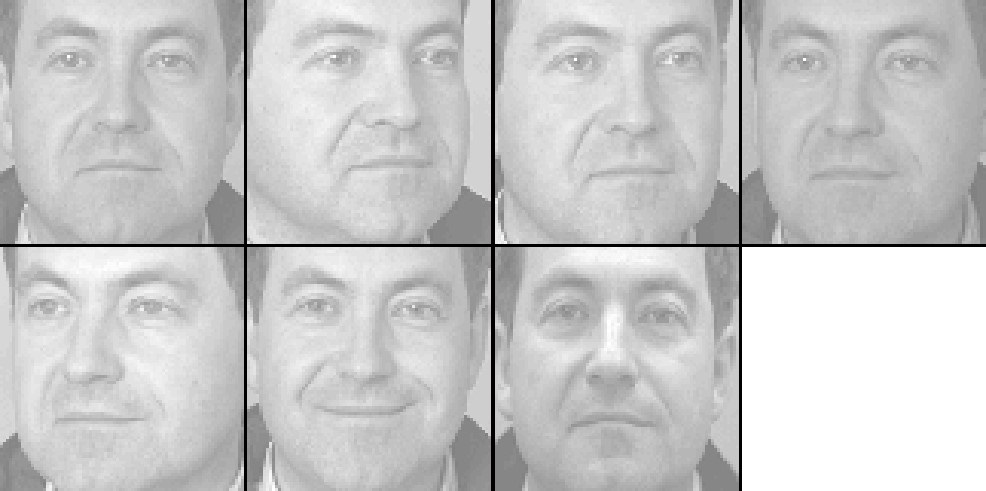
\includegraphics[width=10cm]{face.jpg}
    \caption{FERET数据示例}
    \label{face-sample}
\end{figure}
\par 在预处理部分,通过调用drtoolbox的降维函数来对数据集($1400\times 6400$)进行降维处理得到“特征脸”($1400\times 100$)。
\begin{lstlisting}
[mappedX, mapping] = compute_mapping(X, 'PCA', 100);
\end{lstlisting}
\par 本实验中使用网格寻优法来寻找最佳的参数c和g。网格寻优法是在给定参数c和g的范围基础上,指定svmtrain的-v参数为5,然后对每一个可能的c和g进行训练得到最优分类。如下面这段代码所示:
\begin{lstlisting}
svmtrain(train_label,train_matrix,'-t 2 -c 1.0 -g 0.1 -v 5');
\end{lstlisting}
其中,-t参数表示核函数选择,2为高斯核;-v参数表示k-fold验证。

\par 主程序代码如下:
\begin{lstlisting}
%  Load Face dataset
load ('face_pca.mat')
X = M(:,1:100);
Y = M(:,101);
%缩放
[X_norm, mu, sigma] = featureNormalize(X);

trainSetX = X_norm(1:1200,:);
trainSetY = Y(1:1200,:);
testSetX = X_norm(1201:1400,:);
testSetY = Y(1201:1400,:);
%网格寻优,交叉验证
cmd = grid_parameter(trainSetY,trainSetX,cmd);
cmd
%模型训练
model = svmtrain(trainSetY,trainSetX,cmd);
model
Parameters = model.Parameters
%预测
[ptrain,acctrain,dec_values] = svmpredict(trainSetY,trainSetX,model);
[predictlabel,accuracy,dec_values] = svmpredict(testSetY,testSetX,model);
\end{lstlisting}
\subsection*{实验结果}
\par 在实验过程中,先后应用了线性核和高斯核进行训练,利用k-fold(其中k=5)选择最优的参数c和g,得到的结果如下表。
\begin{table}[!hbp]
\centering
\begin{tabular}{|c|c|c|c|c|}
\hline
\hline
 核函数 &  c &  g &  训练精度 &  预测精度 \\
\hline
 线性核 &  0.03125 &  1.0 & 97.0$\%$  &  80$\%$ \\
\hline
 高斯核 &  32 &  0.00003051 &  93.75$\%$ &  77$\%$ \\
\hline
\hline
\end{tabular}
\caption{实验结果}
\end{table}
\newpage
\section*{不同种类的SVM}
\subsection*{$\upsilon$-SVM}
\par 在SVM中,通过参数C实行对错误分类的惩罚,但如何选择C并没有直观的解释。在$\upsilon$-SVM方法中,优化问题为
\begin{eqnarray}     
\left.            
\begin{array}{ccc}     
min_{w,b,\xi }\frac{1}{2}\left \| w \right \|^{2}-\upsilon\rho +\frac{1}{l}\sum_{i=1}^{l}\xi _{i} \\
s.t.\; \; y_{i}(w\cdot \phi (x_{i})+b)\leq \rho -\xi _{i}\\   
\xi _{i}\geq 0\\
\rho > 0
\end{array}          
\right\}         
\end{eqnarray} 
\par 其对偶形式为
\begin{eqnarray}     
\left.            
\begin{array}{ccc}     
max_{\alpha} \left \{ L_{D}=-\frac{1}{2}\sum_{i=l}^{l}\sum_{j=l}^{l})\alpha _{i} \alpha _{j} y_{i} y_{j}K(x_{i},x_{j}) \right \}\\
s.t.\; \; 0\leq \alpha _{i}\leq \frac{1}{l} \\
\sum_{i=1}^{l}\alpha _{i}y_{i}=0\\   
\sum_{i=1}^{l}\alpha _{i}\geq \nu
\end{array}          
\right\}         
\end{eqnarray} 
\par 由KKT条件知,在最优点满足
$$\sum_{i=1}^{l}\alpha _{i}= \nu$$
\par 对于边界支持向量,$\alpha_{i}=1/l$,因此对于$N_{BSV}$个边界支持向量有$$(N_{BSV}\setminus l)\leq \sum_{i=1}^l{}\alpha _{i}=\nu$$ 而对于支持向量,$\alpha_{i} \leq 1 \setminus l$,因此对于$N_{SV}$个支持向量有$\sum_{i=1}^l{}\alpha _{i}\leq N_{SV}\setminus l$,即$N_{SV}\setminus l \geq \nu $,因此有
$$N_{BSV}\setminus l \geq \nu \leq N_{SV}\setminus l$$
\par 可以看出,$\upsilon$-SVM中参数$\upsilon$的物理意义非常明确,$l、v$表示BSV数量的上限和SV数量的下限。
\subsection*{LS-SVM}
\par 在最小二乘支持向量机中,优化指标采用了平方项,从而将不等式转变为等式约束,最优化问题为
\begin{eqnarray}     
\left.            
\begin{array}{ccc}     
min_{w,b,\xi }\frac{1}{2}\left \| w \right \|^{2} +\frac{1}{2}r \sum_{i=1}^{l}\xi _{i} \\
s.t.\; \; y_{i}(w\cdot \phi (x_{i})+b) = 1 -\xi _{i}
\end{array}          
\right\}         
\end{eqnarray} 
可得到线性方程组
\begin{equation}       
\left[                
  \begin{array}{ccc}   
    0 & y^{T}\\  
    y & Q+r^{-1}I\\  
  \end{array}
\right]_{(l+1)\times(l+1)}
\left[                
  \begin{array}{ccc}   
    b\\  
    \alpha\\  
  \end{array}
\right]=
\left[                
  \begin{array}{ccc}   
    0\\  
    e\\  
  \end{array}
\right]                
\end{equation}
式中:$e\in R^{l}$是元素为$l$的向量;$I\in R^{l\times l}$为单位阵;$\alpha=[\alpha_{1},\alpha_{2},\cdots ,\alpha_{l}]^{T}\in R^{l}$;$y=[y_{1},y_{2},\cdots ,y_{l}]^{T}\in R^{l}$;$Q=[q_{ij}]_{l\times l}$;$q_{ij}=y_{i}y_{j}K(x_{i},x_{j})$。在LS-SVM中,将二次规划问题转变为线性方程组的求解,简化了计算复杂度。但由于每个样本数据对分类器都有贡献,LS-SVM失去了稀疏性的优点。
\subsection*{W-SVM}
\par 在SVM中,引入惩罚参数C实行对错误分类的惩罚。在实际应用中,某些重要样本正确分类的要求高,而某些样本正确分类的要求低,因此,在优化问题描述中,对每个采样点数据采用不同的惩罚系数,以得到更准确的分类,这种支持向量机称之为加权支持向量机。另外,不同类别的样本数量差异比较大时,存在着分类结果偏向于多项本类别的问题,这类问题的解决方法本质上也是W-SVM。W-SVM的最优化问题描述为
\begin{eqnarray}     
\left.            
\begin{array}{ccc}     
min_{w,b,\xi }\frac{1}{2}\left \| w \right \|^{2} +\frac{1}{2}s_{i} \sum_{i=1}^{l}\xi _{i}\\
s.t.\; \; y_{i}(w\cdot \phi (x_{i})+b) \geq  1 -\xi _{i}\\
\xi _{i}\geq 0,i=1,2,\dots,l
\end{array}          
\right\}         
\end{eqnarray} 
\par $\xi_{i}$为加权系数,对偶最优化问题为
\begin{eqnarray}     
\left.            
\begin{array}{ccc}     
max_{\alpha} \left \{ L_{D}=\sum_{i=1}^{l}\alpha_{i}-\frac{1}{2}\sum_{i=l}^{l}\sum_{j=l}^{l})\alpha _{i} \alpha _{j} y_{i} y_{j}K(x_{i},x_{j}) \right \} \\
s.t.\; \; 0\leq \alpha _{i}\leq Cs_{i} \\
\sum_{i=1}^{l}\alpha _{i}y_{i}=0
\end{array}          
\right\}         
\end{eqnarray} 
\newpage
\section*{parzen窗概率密度估计}
\par parzen窗是一种非参数估计概率密度的方法。已知N数据,不知道它的分布情况,估计它的概率密度
$p(x)\approx \frac{1}{Nh^{l}}\sum_{i=1}^{N}\phi (\frac{x-x_{i}}{h})$
\par 其中N为样本数量,h为窗长度,$phi(\dot)$为核函数。
\begin{lstlisting}
function  parzen()
clc;
N = 256;                           %样本个数.
x = linspace(-3, 3, 100); 
f = rand(N, 1); 
X = zeros(N, 1); 
 
for i = 1:N                        %生成样本矩阵X.
   if f(i)<0.5 
       X(i) = 2*(f(i)-1); 
   else 
       X(i) = 2*f(i); 
    end 
end

p = Parzen(x, X, 0.25, 1);     
subplot(3,3,1);plot(x, p);
title('N =1, h1 = 0.25');axis([-3, 3, 0, 1.5]);
p = Parzen(x, X, 1, 1);        
subplot(3,3,4);plot(x, p);
title('N =1, h1 = 1');axis([-3, 3, 0, 1.5]); 
p = Parzen(x, X, 4, 1);        
subplot(3,3,7);plot(x, p);
title('N =1, h1 = 4');axis([-3, 3, 0, 1.5]); 
p = Parzen(x, X, 0.25, 16);   
subplot(3,3,2);plot(x, p);
title('N =16, h1 = 0.25');axis([-3, 3, 0, 1.5]); 
p = Parzen(x, X, 1, 16);      
subplot(3,3,5);plot(x, p);
title('N =16, h1 = 1');axis([-3, 3, 0, 1.5]); 
p = Parzen(x, X, 4, 16);       
subplot(3,3,8);plot(x, p);
title('N =16, h1 = 4');axis([-3, 3, 0, 1.5]); 
p = Parzen(x, X, 0.25, 256);   
subplot(3,3,3);plot(x, p);
title('N =256, h1 = 0.25');axis([-3, 3, 0, 1.5]); 
p = Parzen(x, X, 1, 256);      
subplot(3,3,6);plot(x, p);
title('N =256, h1 = 1');axis([-3, 3, 0, 1.5]); 
p = Parzen(x, X, 4, 256);      
subplot(3,3,9);plot(x, p);
title('N =256, h1 = 4');axis([-3, 3, 0, 1.5]); 
end
 
function p = Parzen(x, X, h1, N)  % x为横坐标; X为样本; h1用来调节窗宽h; N为样本个数.
    h = h1 / sqrt(N);           % h为窗宽. 
    sum = zeros(1, 100); 
    for i = 1:N 
        sum = sum + normpdf((x - X(i))/h, 0, 1);     %用正态窗函数作Parzen窗估计
    end 
    p = sum/(N * h); 
end 
\end{lstlisting}
\begin{figure}[h!]
    \centering
    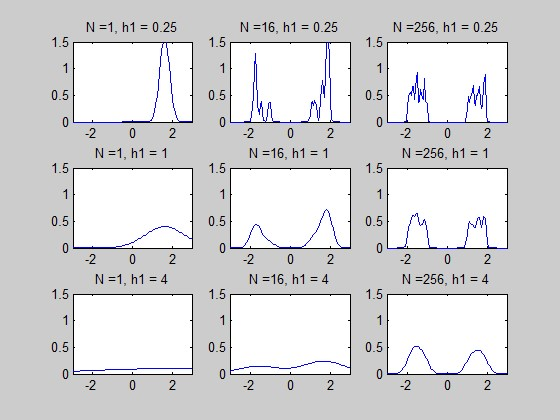
\includegraphics[width=10cm]{Sample.jpg}
    \caption{parzen仿真结果}
    \label{fig-sample}
\end{figure}
\newpage
\section*{深度学习}

\par 机器学习技术在现代社会的各个方面表现出了强大的功能:从Web搜索到社会网络内容过滤,再到电子商务网站上的商品推荐都有涉足。并且它越来越多地出现在消费品中,比如相机和智能手机。

\par 机器学习系统被用来识别图片中的目标,将语音转换成文本,匹配新闻元素,根据用户兴趣提供职位或产品,选择相关的搜索结果。逐渐地,这些应用使用一种叫深度学习的技术。传统的机器学习技术在处理未加工过的数据时,体现出来的能力是有限的。几十年来,想要构建一个模式识别系统或者机器学习系统,需要一个精致的引擎和相当专业的知识来设计一个特征提取器,把原始数据(如图像的像素值)转换成一个适当的内部特征表示或特征向量,子学习系统,通常是一个分类器,对输入的样本进行检测或分类。特征表示学习是一套给机器灌入原始数据,然后能自动发现需要进行检测和分类的表达的方法。深度学习就是一种特征学习方法,把原始数据通过一些简单的但是非线性的模型转变成为更高层次的,更加抽象的表达。通过足够多的转换的组合,非常复杂的函数也可以被学习。对于分类任务,高层次的表达能够强化输入数据的区分能力方面,同时削弱不相关因素。比如,一副图像的原始格式是一个像素数组,那么在第一层上的学习特征表达通常指的是在图像的特定位置和方向上有没有边的存在。第二层通常会根据那些边的某些排放而来检测图案,这时候会忽略掉一些边上的一些小的干扰。第三层或许会把那些图案进行组合,从而使其对应于熟悉目标的某部分。随后的一些层会将这些部分再组合,从而构成待检测目标。深度学习的核心方面是,上述各层的特征都不是利用人工工程来设计的,而是使用一种通用的学习过程从数据中学到的。

\par 深度学习正在取得重大进展,解决了人工智能界的尽最大努力很多年仍没有进展的问题。它已经被证明,它能够擅长发现高维数据中的复杂结构,因此它能够被应用于科学、商业和政府等领域。除了在图像识别、语音识别等领域打破了纪录,它还在另外的领域击败了其他机器学习技术,包括预测潜在的药物分子的活性、分析粒子加速器数据、重建大脑回路、预测在非编码DNA突变对基因表达和疾病的影响。也许更令人惊讶的是,深度学习在自然语言理解的各项任务中产生了非常可喜的成果,特别是主题分类、情感分析、自动问答和语言翻译。我们认为,在不久的将来,深度学习将会取得更多的成功,因为它需要很少的手工工程,它可以很容易受益于可用计算能力和数据量的增加。目前正在为深度神经网络开发的新的学习算法和架构只会加速这一进程。
\subsection*{深度学习基本思想}
\par 假设我们有一个系统$S$,它有$n$层$(S_1,\dots,S_n)$,它的输入是$I$,输出是$O$,形象地表示为: $I\Rightarrow S_1\Rightarrow S_2 \Rightarrow \dots \Rightarrow S_n \Rightarrow O$,如果输出$O$等于输入$I$,即输入$I$经过这个系统变化之后没有任何的信息损失。设处理$a$信息得到b,再对$b$处理得到$c$,那么可以证明:$a$和$c$的互信息不会超过$a$和$b$的互信息。这表明信息处理不会增加信息,大部分处理会丢失信息。保持了不变,这意味着输入I经过每一层$S_i$都没有任何的信息损失,即在任何一层$S_i$,它都是原有信息(即输入$I$)的另外一种表示。我们需要自动地学习特征,假设我们有一堆输入$I$(如一堆图像或者文本),假设我们设计了一个系统$S$(有$n$层),我们通过调整系统中参数,使得它的输出仍然是输入$I$,那么我们就可以自动地获取得到输入I的一系列层次特征,即$S_1,\dots,S_n$。

\par 对于深度学习来说,其思想就是对堆叠多个层,也就是说这一层的输出作为下一层的输入。通过这种方式,就可以实现对输入信息进行分级表达了。

\par 另外,前面是假设输出严格地等于输入,这个限制太严格,我们可以略微地放松这个限制,例如我们只要使得输入与输出的差别尽可能地小即可,这个放松会导致另外一类不同的深度学习方法。上述就是深度学习的基本思想。
\subsection*{深度学习与神经网络}
\par 深度学习是机器学习研究中的一个新的领域,其动机在于建立、模拟人脑进行分析学习的神经网络,它模仿人脑的机制来解释数据,例如图像,声音和文本。深度学习是无监督学习的一种。

\par 深度学习的概念源于人工神经网络的研究。含多隐层的多层感知器就是一种深度学习结构。深度学习通过组合低层特征形成更加抽象的高层表示属性类别或特征,以发现数据的分布式特征表示。

\par 深度学习本身算是机器学习的一个分支,简单可以理解为神经网络的发展。大约二三十年前,神经网络曾经是ML领域特别火热的一个方向,但是后来确慢慢淡出了,原因包括以下几个方面:
\begin{enumerate}[\indent 1)]
\item 比较容易过拟合,参数比较难tune,而且需要不少trick;

\item 训练速度比较慢,在层次比较少(小于等于3)的情况下效果并不比其它方法更优;
\end{enumerate}
\par 所以中间有大约20多年的时间,神经网络被关注很少。但是,Hinton坚持了下来,并最终提成了一个实际可行的深度学习框架。

\par 深度学习与传统的神经网络之间有相同的地方也有很多不同。二者的相同在于深度学习采用了神经网络相似的分层结构,系统由包括输入层、隐层(多层)、输出层组成的多层网络,只有相邻层节点之间有连接,同一层以及跨层节点之间相互无连接,每一层可以看作是一个logistic regression模型;这种分层结构,是比较接近人类大脑的结构的。
\begin{figure}[h!]
    \centering
    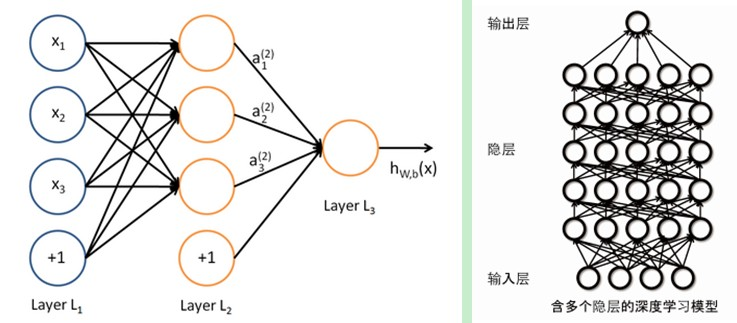
\includegraphics[width=10cm]{0507-3.jpg}
    \caption{神经网络与深度学习}
    \label{fig-sample}
\end{figure}
\par为了克服神经网络训练中的问题,深度学习采用了与神经网络很不同的训练机制。传统神经网络中,采用的是后向传播的方式进行,简单来讲就是采用迭代的算法来训练整个网络,随机设定初值,计算当前网络的输出,然后根据当前输出和label之间的差去改变前面各层的参数,直到收敛(整体是一个梯度下降法)。而深度学习整体上是一个layer-wise的训练机制。这样做的原因是因为,如果采用后向传播的机制,对于一个深度网络(7层以上),残差传播到最前面的层已经变得太小,出现所谓的梯度扩散。
\subsection*{深度学习训练过程}
\par 2006年,hinton提出了在非监督数据上建立多层神经网络的一个有效方法,简单的说,分为两步,一是每次训练一层网络,二是调优,使原始表示$x$向上生成的高级表示$r$和该高级表示$r$向下生成的$x'$尽可能一致。方法是:
\begin{enumerate}[\indent 1)]
\item 首先逐层构建单层神经元,这样每次都是训练一个单层网络。

\item 当所有层训练完后,Hinton使用wake-sleep算法进行调优。
\end{enumerate}
\par 将除最顶层的其它层间的权重变为双向的,这样最顶层仍然是一个单层神经网络,而其它层则变为了图模型。向上的权重用于“认知”,向下的权重用于“生成”。然后使用Wake-Sleep算法调整所有的权重。让认知和生成达成一致,也就是保证生成的最顶层表示能够尽可能正确的复原底层的结点。比如顶层的一个结点表示人脸,那么所有人脸的图像应该激活这个结点,并且这个结果向下生成的图像应该能够表现为一个大概的人脸图像。Wake-Sleep算法分为醒(wake)和睡(sleep)两个部分。
\begin{enumerate}[\indent 1)]
\item wake阶段:认知过程,通过外界的特征和向上的权重(认知权重)产生每一层的抽象表示(结点状态),并且使用梯度下降修改层间的下行权重(生成权重)。也就是“如果现实跟我想象的不一样,改变我的权重使得我想象的东西就是这样的”。

\item sleep阶段:生成过程,通过顶层表示(醒时学得的概念)和向下权重,生成底层的状态,同时修改层间向上的权重。也就是“如果梦中的景象不是我脑中的相应概念,改变我的认知权重使得这种景象在我看来就是这个概念”。
\end{enumerate}
\par 深度学习训练过程具体如下:
\begin{enumerate}[\indent 1)]
\item 使用自下上升非监督学习。采用无标定数据分层训练各层参数,这一步可以看作是一个无监督训练过程,是和传统神经网络区别最大的部分。具体的,先用无标定数据训练第一层,训练时先学习第一层的参数,由于模型容量的限制以及稀疏性约束,使得得到的模型能够学习到数据本身的结构,从而得到比输入更具有表示能力的特征;在学习得到第$n-1$层后,将n-1层的输出作为第$n$层的输入,训练第$n$层,由此分别得到各层的参数;

\item 自顶向下的监督学习。基于第一步得到的各层参数进一步fine-tune整个多层模型的参数,这一步是一个有监督训练过程;第一步类似神经网络的随机初始化初值过程,由于深度学习的第一步不是随机初始化,而是通过学习输入数据的结构得到的,因而这个初值更接近全局最优,从而能够取得更好的效果;所以深度学习效果好很大程度上归功于第一步的特征学习过程。
\end{enumerate}
\end{document}
